%==============================================================================%
%                               RAPPORT DE STAGE                               %
%==============================================================================%
% Auth: Rémi CHASSAGNOL                                                        %
% Desc: Rapport de stage de deuxième année à l'école l'ISIMA.                  %
%==============================================================================%

% Settings ---------------------------------------------------------------- {{{
\documentclass[a4paper]{article}

\usepackage[utf8]{inputenc}
\usepackage[T1]{fontenc}
\usepackage{textcomp}
\usepackage{url}
\usepackage{hyperref}
\usepackage[top=2.5cm,bottom=2.5cm,right=2cm,left=3cm]{geometry}
\usepackage[french]{babel}
\usepackage[backend=biber,style=ieee]{biblatex}
\usepackage{glossaries}
%\usepackage{titletoc}% http://ctan.org/pkg/titletoc
\usepackage{qtree}
\usepackage{listings}
\usepackage{xcolor}
\usepackage{setspace}
\usepackage{graphicx}
\usepackage{geometry}
\usepackage{titlesec}
\usepackage{chngcntr}
\counterwithin*{section}{part}

\addbibresource{refs.bib}

\definecolor{codegreen}{rgb}{0,0.6,0}
\definecolor{codegray}{rgb}{0.5,0.5,0.5}
\definecolor{backcolour}{rgb}{0.95,0.95,0.92}
\definecolor{backpink}{rgb}{1,0.94,0.95}

%===========style & geometry===========
%\lstset{style=mystyle}

 \geometry{
 a4paper,
  left=30mm,
  right=20mm,
  top=25mm,
  bottom=25mm,
 }

 \titleformat*{\section}{\LARGE\bfseries}
 \titleformat*{\subsection}{\Large\bfseries}

%================infos=================
\pagenumbering{gobble}
\begin{titlepage}

\title{Création d'un outil d'intégration continue}
\author{CHASSAGNOL Rémi}
\date{\today}
\end{titlepage}
%}}}
% Glossaire --------------------------------------------------------------- {{{
\makeglossaries
\newglossaryentry{ast}
{
    name=todo,
    description={le truc à faire}
}

%}}}

%------------------------------------------------------------------------------%
%                                   Document                                   %
%------------------------------------------------------------------------------%

\pagestyle{empty}
\begin{document}

% Title page -------------------------------------------------------------- {{{
\begin{titlepage}
  \hspace{\fill}
  \begin{figure}[!htb]
     \begin{minipage}{0.50\textwidth}
       \centering
       
\includegraphics[scale=0.8]{./img/logo_isima_inp.jpeg}
     \end{minipage}\hfill
     \begin{minipage}{0.50\textwidth}
       \centering
       
\includegraphics[scale=0.4]{./img/logo-ck.png}%
     \end{minipage}
  \end{figure}
  \begin{center}
    \vspace*{1cm}

    \par\noindent\rule{\textwidth}{0.5pt}
    \Huge
    \textbf{Création d'un outil d'intégration continue}
    \par\noindent\rule{\textwidth}{0.5pt}

    \vspace{0.2cm}
    \LARGE
    Rapport d'élève ingénieur\\
    Stage de $2^{ème}$ année\\
    Filière F2 : Génie Logiciel et Systèmes Informatiques

    \vspace{1.5cm}

    \large
    Présenté par : \textbf{Rémi CHASSAGNOL}

    \vfill

    \vspace{0.5cm}
  \end{center}


  \large
  \noindent
  Responsable ISIMA : Loïc YON \hfill \textbf{Soutenance: 30/08/2023}\\
  Responsable entreprise : Ludovic DESCOUT \hfill \textbf{Durée du stage: 5 mois}\\~\\
  \raggedright
  \begin{center}
  Campus des Cézeaux. 1 rue de la Chébarde. TSA 60125. 63178 Aubière CEDEX\\
  \end{center}
\end{titlepage}

\clearpage{}

%---------------------------------------------------------------------------}}}
% Table of Content -------------------------------------------------------- {{{
\pagenumbering{arabic}
\thispagestyle{empty}
\tableofcontents
\clearpage{}

%---------------------------------------------------------------------------}}}
% Remerciements ------------------------------------------------------------{{{
\section*{Remerciements}
\thispagestyle{empty}
\addcontentsline{toc}{section}{Remerciements}

\doublespacing

Les remerciements !!

\onehalfspacing

\clearpage{}

%---------------------------------------------------------------------------}}}
% Table des figures --------------------------------------------------------{{{
\listoffigures
\clearpage{}

%---------------------------------------------------------------------------}}}
% Résumé & Abstract --------------------------------------------------------{{{
%\setcounter{secnumdepth}{3}
\section*{Résumé}
\addcontentsline{toc}{section}{Résumé}

Le super résumer !
\\~\\

\noindent
Mots-clés : \textbf{C/C++}, \textbf{intégration continue}, \textbf{tests},
\textbf{systèmes embarqués}, \textbf{émulation}

\section*{Abstract}
\addcontentsline{toc}{section}{Abstract}

the amazing abstract
\\~\\

\noindent
Keywords : \textbf{C/C++}, \textbf{continuous integration}, \textbf{testing},
\textbf{embeded system}, \textbf{emulation}

\clearpage{}

%---------------------------------------------------------------------------}}}
% Introduction -------------------------------------------------------------{{{
\pagestyle{plain}
\setcounter{page}{1}
\clearpage
\section*{Introduction}
\addcontentsline{toc}{section}{Introduction}

Introduction

plan !

\clearpage{}

%---------------------------------------------------------------------------}}}

%------------------------------------------------------------------------------%
%                                     Plan                                     %
%------------------------------------------------------------------------------%

% Contexte du projet *******************************************************{{{
\part{Contexte du projet}

\section{Présentation de CKsquare}

CKsquare est une entreprise d'ingénierie spécialisée dans la conception de
systèmes de payement automatisés.

L'entreprise fourni principalement les stations de lavage automatiques pour les
voitures ainsi que les laveries mais s'intéresse aussi à d'autre marchés. Par
exemple, elle est en train de mettre en place un projet projet de casier
entièrement automatisés qui pourront être utilisés pour acheter des produits
locaux.

CKsquare est un groupe composé de plusieurs sociétés chacune chargé de la
conception d'une partie des borne. Cela permet de faire en sorte que la
fabrication des bornes soit presque entièrement réalisé par l'entreprise.

% TODO: revoir cette partie
L'objectif de la société est de pouvoir fournir des produits configurables et
adaptables aux besoins des différents clients. Une équipe SAV est en permanence
à l'écoute des requêtes des clients ce qui permet de guider l'équipe de
développement pour la conception d'éléments permettant de répondre à ces
besoins.

% aspect sécurité ?
% je suis pas encore satisfait de ce paragraphe
Un des gros atouts de la société est son savoir faire concernant l'utilisation
des cartes électroniques. En effet, les bornes CKsquare sont toutes équipées de
cartes électroniques beaucoup plus fiables et moins énergivores que des PC.
Cependant, ces cartes doivent assurer beaucoup de fonctionnalités et gérer un
grand nombre de composants ce qui pose de gros problèmes en terme d'optimisation
du stockage. De plus, l'utilisation d'outils de payements implique encore plus
de contraintes comme par exemple la nécessité de s'assurer que toutes les ventes
sont correctement enregistrées puis envoyées sur le serveur.

- monétique ++
- station auto lavage
- faite ses 20 ans cette année
- pousse les carte électroniques très loin -> solution très fiable / économique
  et écologique
- ils ont mis en place des systèmes perso pour pousser les cartes encore plus
  loin
- regroupement d'entreprises pour concevoir les bornes de A à Z
- fournissent des solution personnalisées pour les clients

\section{Travail demandé}

L'objectif est de réaliser un outil servant à faire de l'intégration continu
pour valider les fichier de la partie commune du code utilisé sur les bornes.
L'outil doit permettre l'écriture de tests pour valider le code et doit pouvoir
être automatisé dans une pipeline Gitlab. De plus, l'outil sera utilisé pour
tester du code exécuté sur du matériel embarqué, il faudra donc un moyen de
tester des fonctions qui interagissent avec le matériel électronique. Pour ce
faire, il faudra émuler les interactions avec le matériel en créant des
fonctions et des structures de données qui réagiront comme les composants
électroniques. Par exemple, si une fonction doit modifier un registre sur une
carte, il faut pouvoir émuler l'interface de la carte et le registre pour
vérifier que les bonnes modification ont été apportées. Il faudra aussi des
fonctionnalités permettant de simuler l'interaction d'un utilisateur avec un
composant pendant les tests. Par exemple, on doit pouvoir faire en sorte de
tester le comportement du système lorsqu'un utilisateur appuie sur une séquence
de touches.

Il sera donc nécessaire d'émuler la mémoire des composants électroniques les
fonctions qui permettent d'interagir avec ainsi que des fonctions permettant de
simuler les actions d'un utilisateur.

La première tâche sera de trouver le framework de test adapté pour la conception
de l'outil. Le code à tester est écrit en C, cependant, la société souhaiterait
aussi pouvoir tester les bibliothèques écrites par l'équipe Qt. Il serait donc
intéressant que l'outil soit aussi adapté au C++.

Étant donné que les tests seront exécuter dans une pipeline (donc dans un
docker), il faudra s'assurer que le code puisse compiler sous Linux. De plus, le
code étant à la base fait pour s'exécuter sur une carte électronique, cela
nécessitera d'émuler les composants pour que le code puisse fonctionner
correctement. Il sera aussi nécessaire de simuler les interfaces permettant au
code d'interagir avec les composants émulés en utilisant différents protocoles
de communication comme le SPI ou encore le Cctalk. En plus de cela, il faudra
pouvoir remplacer une partie des bibliothèques de la carte pour pouvoir simuler
les composants.

Le résultat final doit être un outil qui doit pouvoir être facilement
réutilisable et adaptable. La documentation et la structure du code doit pouvoir
permettre d'aisément modifier ou copier les différents éléments. Par exemple, il
faudra que tous les composants simulés aient la même structure et que cette
structure soit suffisamment simple et générique pour pouvoir être copiée pour la
création d'un nouveau composant.

À noter que l'objectif du projet n'est pas d'écrire des tests. Des tests ont été
écrits durant le projet mais ces derniers ont pour objectif de valider le bon
fonctionnement des composants simulés et non celui du code de la société.

\clearpage
%***************************************************************************}}}
% Réalisation et conception ************************************************{{{
\part{Réalisation et conception}

\section{Choix du framework de test}

Le but du projet est de concevoir un outil permettant de tester du code, la
première tâche à donc été de choisir un framework de test. Le framework de test
constitue la base de l'outil à créer, c'est donc un choix assez important. Dans
cette partie nous traiterons de la procédure qui a été utilisée pour trouver et
comparer des frameworks et des bibliothèques de test.

\subsection{Les critères de comparaison}

Étant donné le fait que le langage C est très utilisé, il y a beaucoup de choix
quand aux différentes bibliothèques de test utilisables. Le premier travail a
été de faire un listing des bibliothèques et frameworks de tests existants pour
ensuite pouvoir les comparer. Ce travail de recherche à permis de faire un prés
tri et d'éliminer les framework incomplets ou trop peut utilisés. Une fois le
listing terminé, il a fallut trouver des critères pour comparer les frameworks.

Tout d'abord, l'équipe de développement souhaitait pouvoir tester à la fois du
code \textbf{C} et du code \textbf{C++} pour pouvoir tester certaines parties de
code développées par l'équipe \textbf{Qt}. Ce critère était optionnel mais
apprécié. À noter que lorsque l'on parle de pouvoir tester du code C++, cela ne
prend pas seulement en compte le fait de pouvoir exécuter des fonctions basiques
puisque c'est parfaitement possible avec tous les frameworks C étant donné la
compatibilité entre le C et le C++. Pour pouvoir tester du code C++, il fallait
aussi que le framework soit capable d'interagir avec les structures de donnés
fournis par la bibliothèque standard de C++ ou encore de pouvoir traiter des
exceptions. Ce critère à aussi été considéré pour la recherche du framework et
des frameworks C++ on aussi été retenus..

Un autre critère concerne la modernité et la facilité d'utilisation du
framework. Cela peut sembler anodin mais l'écriture des tests est une tâche
aussi longue que le développement. Pour ne pas perdre de temps, il est
préférable que les tests soient le plus simple possible à mettre en place. De
plus, les tests peuvent aussi servir de documentation, c'est donc un avantage
non négligeable que d'avoir un framework qui permette d'écrire des tests
simples, lisibles et compréhensibles. Enfin, ce critère impacte aussi le temps
de conception de l'outil de test car le fait d'utiliser un framework trop
complexe aurait nécessité la conception de fonctions et macros (pour réduire la
complexité) et rallongé le temps d'écriture de la documentation. À noter que
pour valider ce critère, la documentation des différents outils a aussi été
étudiée, les frameworks devaient donc fournir une documentation suffisamment
claire et précise permettant d'utiliser facilement toutes les fonctionnalités
proposées.

% TODO: reformuler
Le critère le plus important est celui du statut du développement du framework.
En effet, lorsque l'on souhaite utiliser un outil, une question importante à se
poser est de savoir ce que l'on peut faire en cas de problème. Ici, il a fallut
regarder la taille, la popularité et l'age des projets. En effet, plus un projet
est populaire plus il sera facile de trouver de l'aide en cas de problème. De
plus, les projet important on souvent beaucoup plus de collaborateurs ce qui
peut accélérer la corrections des bugs. Enfin la dates de dernières mis à jours
ont aussi été répertoriées car là aussi, il est beaucoup plus simple de résoudre
les problèmes sur un projet qui est encore activement maintenu.

% TODO: mal dit
D'autres critères ont permis de démarquer les frameworks comme par exemple le
fait que les frameworks fournisse des fonctionnalités supplémentaires comme le
fait de pouvoir exporter les résultats des tests dans différents format comme
TAP ou XML (utile pour faire des rapport) ou encore des générateur de nombres
pseudo aléatoires pour faire des tests avec des entrée aléatoires, \dots Une
autre fonctionnalité intéressante est que les frameworks exécutent les tests
dans des threads séparer ce qui permet de tester des signaux ou encore de ne pas
stopper tous les tester pour un plantage.

% TODO: résumé des frameworks

\section{Organisation du projet}

- myosismonnayeur
- fichiers de bases
  - Les fichiers locaux
  - Fichiers à tester (commun\_global, dev\_pic)
- les fichiers de Tests

\section{Simulation du stockage}

Une partie importante de l'émulation concerne le stockage et il y a plusieurs
types composants à simuler, les registres, les eeproms, et la mémoire flash.
L'émulation des périphériques des stockage est assez simple puisqu'il s'agit
simplement de tableaux de caractères non signés (codés sur 8 bits sur la plupart
des machines). La partie complexe de l'émulation du stockage concerne
l'interface qui permet d'interagir avec les périphériques. Il y a deux
protocoles qui sont utilisés avec le stockage. Tout d'abord il y a le protocole
I²C qui est utilisé avec les registre et certaines eeproms. Ensuite il y a le
protocole SPI qui est utilisé avec les eeproms et les mémoire flash.

Dans cette partie nous allons voir comment a été réalisée l'émulation de
l'interface permettant d'utiliser le stockage avec les différents protocoles.

\subsection{Échec des threads}

La première solution qui a été implémentée utilisait des \textbf{threads}.
L'objectif été de pouvoir simuler les composants de sorte à ce qu'ils se
comportent comme les composants réels installés sur la carte. Pour se faire, il
été souhaitable que les composants simulés soient actif en même temps que la
carte (représentée ici par le programme à tester) et c'est pour cela que les
threads ont été utilisés. Le principe était que les composants été représentés
par des machines à états qui bouclaient dans un état de base jusqu'à ce que le
composant soit appelé (donc jusqu'à ce que le programme principale décide de
lancer une communication en utilisant un des protocoles cités précédemment). Une
fois le composant appelé, la machine à états permettait d'assurer la
communication. Pour que les composant simulé s'exécutent en même temps que le
programme principale, la fonction qui contenait la machine à états était
exécutée dans un thread.

\subsection{Interface I²C}


\subsection{Interface SPI}


\section{Simulation des composants}

\subsection{Interface Cctalk}

\subsection{Interface MDB}


\section{Déroulement du projet}

\subsection{Les outils utilisés}

\subsubsection{Gestion de version}

utilisation de git / version modifiée de gitflow. Je suis seul mais j'ai quand
même organiser mes branche de façon similaire à gitflow pour ne jamais casser du
code qui marche en mergant ou en tentant d implémenté du code qui marche pas.

\subsubsection{Gitlab}

ci/cd

\subsubsection{Compilation}

L'objectif étant de pouvoir automatiser les tests dans une pipeline Gitlab, il
fallait obligatoirement que les tests puissent compiler sur un docker et donc
sur un Linux. L'outil le plus adapté pour ce genre de tache est
\textbf{Makefile} qui a été utilisé en début de projet. Le défaut de Makefile
est qu'il reste assez proche du script et qu'il faut obligatoirement détailler
toutes les commandes. Étant donné le fait qu'il y avait beaucoup de fichiers, le
Makefile est vite devenu très compliqué et illisible et ce même si aucune
compilation séparé n'a été mise en place au début du projet. Quand de plus en
plus de fichiers ont été ajoutés au projet de test, il a fallut mettre en place
de la compilation séparée pour ne pas tout recompiler à chaque fois. Faire cela
avec Makefile est tout à fait possible mais cela aurait pris beaucoup de temps     % rep cela
et le fichier final aurait été assez peu lisible et surtout assez compliqué à
comprendre. Le but étant de faire un outil facilement compréhensible et
utilisable par tous les membres de l'entreprise, il fallait trouver une solution
plus simple. La syntaxe de \textbf{CMake} à permis de simplement lister les
fichiers à compiler ainsi que les répertoires à inclure sans avoir besoin de
détailler les option de gcc. Cet outil permet de générer un Makefile complet
avec un syntaxe beaucoup plus simple. De plus, CMake permet nativement de faire
de la compilation séparer ce qui à permis de gagner du temps pendant le
développement étant donner le fait que seuls les fichiers modifiés sont
recompilés lors de l'écriture des tests.

\subsubsection{nvim}

I use vim btw

\subsection{Planification des tâches}

On voit ça sur le gantt.

Ce diagramme est disponible en index \ref{appendix:expectedgantt} pour
plus de lisibilité.

% [expected gantt] {{{
% \begin{figure}[h!]
%   \begin{center}
%   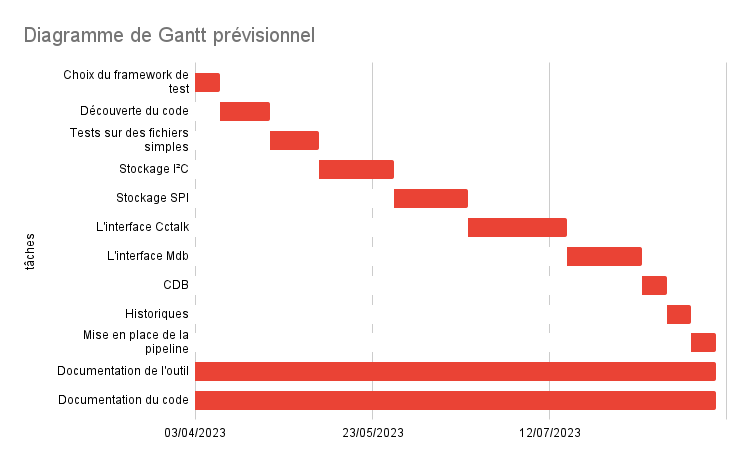
\includegraphics[scale=0.35]{./img/expected-gantt.png}
%   \caption{Diagramme de Gantt prévisionnel}
%   \end{center}
% \end{figure}
%}}}

Mais en fait on a fait ça parceque

On peut retrouver ce diagramme en index \ref{appendix:realgantt}.

% [real gantt] {{{
% \begin{figure}[h!]
%   \begin{center}
%   \includegraphics[scale=0.35]{./img/real-project.png}
%   \caption{Diagramme de Gantt réel.}
%   \end{center}
% \end{figure}~\\
%}}}

conclusion

\clearpage
%***************************************************************************}}}
% Résultats et discussions *************************************************{{{
\part{Résultats et discussions}

\section{TODO}

todo

\clearpage

\section{Discussion et perspectives}

On a fait ça et c'est bien mais on pourrait faire ça ou changer ça.

\clearpage

\section*{Conclusion}
\addcontentsline{toc}{section}{Conclusion}

CONCLUSION

%***************************************************************************}}}

%------------------------------------------------------------------------------%
%                                 bibliography                                 %
%------------------------------------------------------------------------------%

\begin{itemize}
  \item \cite{mankar2014review}: présentation du protocole I²C
  \item \cite{dhaker2018introduction} et \cite{li2014design}: présentation du
    protocole SPI
  \item \cite{engblom2015continuous}: simulation pour CI sur systèmes embarqués
  \item \cite{maartensson2016continuous}: intégration continue sur les systèmes
    embarqués.
  \item \cite{hamill2004unit}: livre sur les frameworks de tests (p 41: mocking)
\end{itemize}

\clearpage{}
\pagestyle{empty}
\printbibliography[keyword={paper},title={Biliographie}]
\printbibliography[keyword={web},title={Webographie}]

%------------------------------------------------------------------------------%
%                                  glossaire                                   %
%------------------------------------------------------------------------------%
\clearpage
\printglossaries

%------------------------------------------------------------------------------%
%                                   annexes                                    %
%------------------------------------------------------------------------------%
\appendix

% Diagramme de Gantt prévisionnel ------------------------------------------{{{
\clearpage{}
\section{Diagramme de Gantt prévisionnel}\label{appendix:expectedgantt}

% \begin{figure}[h!]
%   \begin{center}
%   \rotatebox[origin=c]{90}{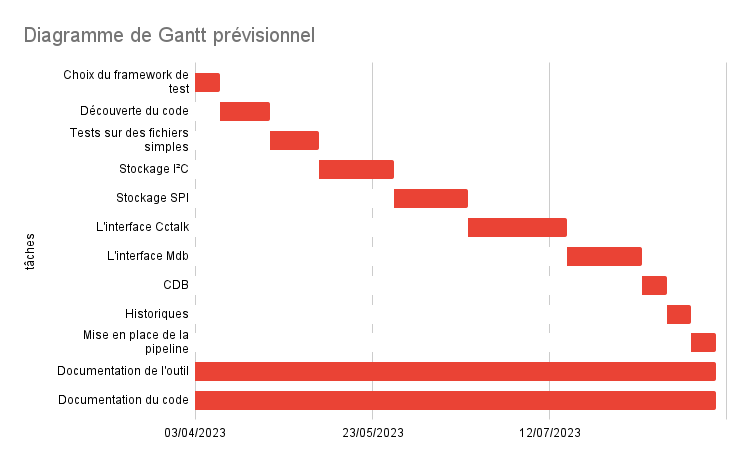
\includegraphics[scale=0.5]{./img/expected-gantt.png}}
%   \caption{Diagramme de Gantt prévisionnel.}
%   \end{center}
% \end{figure}
%---------------------------------------------------------------------------}}}
% Diagramme de Gantt réel --------------------------------------------------{{{
\clearpage{}
\section{Diagramme de Gantt réel}\label{appendix:realgantt}

% \begin{figure}[h!]
%   \begin{center}
%   \rotatebox[origin=c]{90}{\includegraphics[scale=0.5]{./img/real-project.png}}
%   \caption{Diagramme de Gantt réel.}
%   \end{center}
% \end{figure}
%---------------------------------------------------------------------------}}}

\end{document}
